\chapter{Stratified Populations: 
Multi-session and Multi-site Data}
\markboth{Stratified Population Models}{}
\label{chapt.hscr}

\vspace{0.3cm}


In this chapter, we describe SCR models for situations when we have
multiple, distinct groups, strata or ``sessions'' (multi-session
models using the \mbox{\tt secr} terminology). The models are
extremely general and provide a flexible hierarchical modeling
framework for modeling abundance \citep{converse_royle:2012,
  royle_etal:2012arXiv}.  We believe that such ``stratified''
populations are extremely commonplace, yet most SCR applications have
been based on models that are distinctly single-population
models. This is done either by analyzing seperate data sets
one-at-a-time or by pooling data from multiple study areas.  A
standard example that arises frequently is that in which multiple
distinct patches (often refuges, parks or reserves) are sampled
independently with the goal of estimating the population size in each
reserve. It makes sense to combine the data together into a single
model that permits the sharing of information about some parameters,
but provides individual estimates of abundance for each land unit.  A
similar situation is that in which a number of replicate trap arrays
are located within a landscape, sometimes for purposes of evaluating
management actions or landscape structure. This is extremely common in
studies of small mammals \citep{converse_etal:2006jwm,
  converse_etal:2006ea, converse_royle:2012}, or in mist-netting of
birds \citep{desante_etal:1995} (BETTER REF HERE WOULD BE NICE), but
there are examples of large-scale monitoring of carnivores and other
species, e.g., tigers \citep{jhala_etal:2011}.


Stratifed or multi-session SCR models are also directly relevant when
the grouping is based on distinct time samples, either periods within
a biological season, or even across years. 
%Even with a single study
%area or trap array, it would be common to conduct multiple samples
%over short intervals, but then repeat sampling again some weeks or
%months later, and perhaps on multiple years.  
Unlike in the case of having spatial strata, with temporally defined
samples, we imagine a fully dynamic, or demographically open, model
that involves survival and recruitment might be suitable. We deal with
those models specifically in Chapt. \ref{chapt.open}.  However, the
stratified (multi-session) models we deal with in this chapter can be
thought of as a primative type of model for open systems, but in which
the populations are assumed to be {\it independent}. Whereas the
underlying model may be one of Markovian dynamics (survival,
recruitment), we could {\it ignore} that dependence for convenience or
perhaps the dynamics are not distinctly estimable because individual
recapture rate is low.


We focus mostly on Bayesian analysis of stratified SCR models using
data augmentation \citep{royle_etal:2012arXiv,royle_converse:2013}. 
The technical modification of data augmentation to deal with such
models is that it is based on a model for the joint distribution of
the stratum-specific population sizes, 
$N_{g}$, {\it conditioned} on their total. This results in a 
multinomial distribution which we can analyze in some generality using data
augmentation.  As a practical matter, specification of this multinomial
distribution for the $N_{g}$ parameters {\it induces} a distribution
for an individual covariate, say $g_{i}$, which is ``group membership''. 
This is extremely handy to analyze by MCMC in the various {\bf BUGS}
engines that you are familiar with by now.

The {\bf R} package \mbox{\tt secr} fits a class of multi-session
models which we have already seen (sec. \ref{mle.sec.multisession})
and we used this class of models to analyze the ovenbird data in
\mbox{\tt secr} (sec. \ref{poisson-mn.sec.ovenbird}). Later in this
chapter we will provide a Bayesian analysis of the ovenbird data in
{\bf BUGS} using an analogous class of models.










\section{Data Structure}


We suppose that $g=1,2,\ldots,G$ populations, having sizes $N_{g}$,
state-spaces ${\cal S}_{g}$ are sampled using some capture-recapture
method producing sample sizes of $n_{g}$ unique individuals and
encounters $y_{ijk}$ for individual $i=1,2,\ldots, \sum_{g=1}^{G}
n_{g}$.  Right now we won't be concerned with the details of every
type of capture-recapture observation model so, for context, we
consider the Bernoulli model in which individual and trap-specific
encounter frequencies are binomial counts: $y_{ij} \sim
\mbox{Binomial}(K,p_{ij})$.  Let $g_{i}$ be a covariate
(integer-valued, $1, \ldots, G$) indicating the population membership
of individual $i$. This covariate is {\it observed} for the sample of
captured individuals but not for individuals that are not captured.

A key idea that we develop shortly is that 
the assumption of certain models for the collection of abundance variables
$N_{g}$ {\it implies} a specific model for the population membership
variable $g_{i}$.  
Then, the data from all populations can essentially
be pooled, and analyzed as data from a single population with the
appropriate model on $g_{i}$, without having to model the $N_{g}$
parameters {\it directly}. In this way, we can easily build
hierarchical models for stratified populations, using an {\it
  individual} level parameterization of the model. Obviously this is
important for SCR models as they all possess at least onee random
effect in the form of the activity center ${\bf s}$. Moreover, in the
context of stratified or multi-session type models, the ``population
membership'' variable $g_{i}$ is a {\it categorical} type of individual
covariate (Huggins 1989; Alho 1990; Royle 2009).  

To illustrate the prototypical  data structure for stratified SCR data, we suppose that a population
comprised of 4 sub-populations is sampled $K=5$ times. Then a
plausible data set has the following structure:
\begin{verbatim}
      individual (i) : 1  2  3  4  5  6  7  8  9 10  
total encounters (y) : 1  1  3  1  1  2  2  4  1  1
      group (g)      : 1  1  1  2  3  3  3  3  4  4
\end{verbatim}
This data set indicates three individuals were captured in subpopulation 1
(captured 1, 1, and 3 times), a single individual was captured in
population 2, four individuals were captured in population 3, and two
individuals were captured in subpopulation 4.


\section{Multinomial Abundance Models}

The Poisson GLM is commonly used throughout ecology to model variation
in abundance.  Consider sampling $g=1,2,\ldots,G$ populations having
unknown sizes $N_{g}$:
\begin{equation}
 N_{g} \sim \mbox{Poisson}(\lambda_{g})
\label{eq.poisson1}
\end{equation}
with
\begin{equation}
\log( \lambda_{g} ) = \beta_{0} + \beta_{1} x_{g}
\label{eq.poisson2}
\end{equation}
where $x_{g}$ is some measured attribute for population $g$. Under this
Poisson model, by conditioning on the total population size over all
$G$ populations, the $N_{g}$ variables have a multinomial distribution:
\begin{equation}
{\bf N} = (N_{1},\ldots,N_{G}) | \{ N_{T} =
\sum_{g} N_{g} \} \sim \mbox{Multinom}( {\bm \pi} | N_{T}).
\label{eq.mn.N}
\end{equation}
with 
multinomial probabilities $\pi_{g} = \lambda_{g}/\sum_{g}
\lambda_{g}$. This relationship between Poisson and multinomial random
variables is a standard distribution theory result. 


{\bf XXXX below here needs edited and reworked XXXXX}
{\bf XXXX don't need any of this ... just the z/g model cite back to
  R/C papers XXXX}



To devise a data augmentation scheme for this model of population
size, we embed the multinomial for $\{ N_{s} \}$ into a multinomial of
the same dimension but with larger, fixed sample size.  Specifically,
we introduce a latent super-population variable $M_{s}$ which we
assume has the desired Poisson distribution but with scaled mean:
$M_{s} \sim \mbox{Poisson}(A \lambda_{s})$ where $A>>1$ where $A$
exists (can be chosen) to ensure that $M_{s}$ is arbitrarily larger
than $N_{s}$.  Conditional on the total super-population size $M_{T} =
\sum_{s} M_{s}$, then ${\bf M}$ has a multinomial distribution:

\begin{equation}
{\bf M}|M_{T} \sim \mbox{Multinom}(M_{T};  {\bm \pi} ) 
\label{eq.mn1}
\end{equation}
where $\pi_{s} = \lambda_{s}/\sum_{s} \lambda_{s}$ which are the same
probabilities as for the target multinomial for ${\bf N}$. 
This multinomial model for the super-population sizes $M_{s}$ is
equivalent to the following:
\[
 g_{i} \sim \mbox{Categorical}({\bm \pi} )
\]
for $g_{i}; i=1,2,\ldots, M_{T}$.  Given {\bf M} or, equivalently,
$g_{i}$, we specify a model for $\{ N_{g}\}$ that differentiates
between ``real'' and ``pseudo-'' individuals by a Bernoulli sampling
model:
\[
 N_{s} \sim \mbox{Binom}(M_{s} , \psi)
\]
where $\psi \sim \mbox{Uniform}(0,1)$. Bernoulli sampling preserves the
marginal Poisson assumption (Takemura 1999). That is, $N_{s}$ is
Poisson, unconditional on $M_{s}$ and, also, 
conditional on $N_{T} = \sum_{s} N_{g}$, ${\bf N}$ has a multinomial
with probabilities ${\bm \pi}$ and index $N_{T}$.  Note also that
$N_{T} \sim \mbox{Binomom}(M_{T}, \phi)$ which is consistent with data
augmentation applied to total population size $N_{T}$. This binomial
sampling model can be represented, equivalently, by the set of
Bernoulli variables:
\[
 z_{i} \sim \mbox{Bern}(\psi)
\]
for $i=1,2,\ldots,M_{T}$.

The multinomial construction makes it clear that $\psi$ is confounded
with $\exp(\beta_{0})$. By constructing the model conditional on the
total, we lose information about the intercept $\beta_{0}$, but this
is recovered in the data augmentation parameter $\psi$.  One of these
parameters has to be fixed. We can set $\beta_0 = 0$ or else we can
fix $\psi$.  The constraint can be specified by noting that, under the
binomial data augmentation model $\mathbb{E}(N_{T}) = \psi M_{T}$ and, under the
Poisson model, $\mathbb{E}(N_{T}) = \sum_{g} \exp(\beta_{0} + \beta_{1} x_{g})$
and so we can set
\[
 \psi = \frac{1}{M_{T}} \sum_{g} \exp(\beta_{0} + \beta_{1} x_{g}).
\]
The equivalence of $\psi$ and $\beta_{0}$ can be thought of in terms of pooling data
from the different sub-populations. In a model with {\it no} covariates, 
we could pool 
all of the data and estimate a single parameter $\psi$ or $\beta_0$ but not
both. In this sense, 
 pooling data from multiple spatial samples is justifiable (in terms of
sufficiency arguments) under a Poisson assumption on local abundance
(which was noted by Royle 2004b; Royle and Dorazio 2008, sec. 5.5.1).


By introducing the latent $M_{g}$ structure, and the Bernoulli
sampling of $N_{s}$, the model is equivalently represented by the
latent variable pair $(g_{i},z_{i})$ where $g_{i}$ is categorical with
prior probabilities $\pi_{s}$ and $z_{i} \sim Bern(\psi)$.  In
particular, the multinomial assumption for the latent variables
$G_{s}$ is formulated in terms of ``group membership'' for each
individual in the super-population of size $M$ according to:
\[
 g_{i} \sim \mbox{Categorical}\left( {\bm \pi} \right)
\]
with ${\bm \pi} = (\pi_{1}, \ldots, \pi_{S})$ and $\pi_{s} =
\lambda_{s}/(\sum_{s} \lambda_{s})$.  Note that aggregating these $M$
categorical variables yields a set of multinomial variables consistent
with Eq. \ref{eq.mn1}. That is, define $G_{1} = \sum_{i=1}^{M} I(g_{i}
= 1)$, $G_{2} = \sum_{i=1}^{M} I(g_{i} = 2)$, etc., where $I()$ is the
indicator function.  The binomial sampling from the super-population,
%$N_{s} \sim \mbox{Binom}(G_{s}, \psi)$
$N_{T} \sim \mbox{Binom}(M, \psi)$
can be described at the level of the individual also, 
 by introducing the binary
variables $z_{1},\ldots,z_{M}$ such that
\[
 z_{i} \sim \mbox{Bern}(\psi)
\]
where $\psi$ is constrained as noted in the previous section. 
We implement this individual-level formulation of the model in BUGS in
Panel \ref{panel.wbcode}.

A second implementation of the model is suggested by working from
Eq. (\ref{eq.mn.N}) -- we can marginalize $N_{T}$
over the prior  $N_{T} \sim \mbox{Binom}(M, \phi)$ to see that 
the  $(S+1) \times 1$ vector 
$(N_{1},\ldots,N_{S},N_{S+1})$ has, conditional on $M$, 
a multinomial distribution 
with cell probabilities
$\pi_{s}^{+} = \pi_{s} \psi$ for $s=1,2,\ldots,S$  and 
 $\pi_{S+1}^{+} = (1-\psi)$ for the last cell which
 corresponds to individuals of the super-population that are not
 members of any of the $S$ populations that were subject to sampling. 
Thus,
\[
{\bf N}|M \sim \mbox{Multinom}({\bm \pi}^{+}).
\]
where the superscript $+$ here indicates that ${\bm \pi}$ is a larger
version of ${\bm \pi}$ from \ref{eq.mn1}.  In this case,
\begin{equation}
g_{i}  \sim \mbox{Categorical}( {\bm \pi}^{+} ) \mbox{ for
  $i=1,\ldots,M_{T}$}  \label{eq.parm1c}
\end{equation}
The two distinct implementations are shown in 
Panel \ref{panel.wbcode} for an ordinary closed population model
(model $M_{0}$).


\begin{panel}[htp]   
\renewcommand{\baselinestretch}{1.0}
\centering
\rule[0.15in]{\textwidth}{.03in}
\begin{tabular}{cc}
\begin{minipage}{2.75in}
{\small
\begin{verbatim}
model {
# This will show that psi and b0 
#   are confounded. 
  p~ dunif(0,1)
  b0~dnorm(0,.1)
  b1~dnorm(0,.1)
  psi ~ dunif(0,1)
  for(s in 1:S){
    log(lam[s]) <- b0 + b1*x[s]
    gprobs[s]<- lam[s]/sum(lam[1:S])
  }
  for(i in 1:M){
    g[i] ~ dcat(gprobs[])
    z[i] ~ dbern(psi)
   y[i]~ dbin(mu[i],J)
   mu[i] <- z[i]*p
  }
  N <- sum(z[1:M]) 
}
\end{verbatim}
}
\end{minipage}
&
\begin{minipage}{2.75in}
{\small
\begin{verbatim}
model {
# This version constrains psi with 
#   the intercept parameter
  p~ dunif(0,1)
  b0~dnorm(0,.1)
  b1~dnorm(0,.1)
  psi<- sum(lam[])/M
  for(j in 1:K){
    log(lam[j]) <- b0 + b1*x[j]
    gprobs[j]<- lam[j]/sum(lam[1:K])
  }
  for(i in 1:M){
    g[i] ~ dcat(gprobs[])
    z[i] ~ dbern(psi)
   y[i]~ dbin(mu[i],J)
   mu[i] <- z[i]*p
  }
  N <- sum(z[1:M]) 
}
\end{verbatim}
}
\end{minipage}
\end{tabular}
\rule[-0.15in]{\textwidth}{.03in}
\caption{BUGS model specification for a capture-recapture model with
  constant encounter probability and Poisson subpopulation sizes,
  $N_{k}$, with mean depending on a single covariate \mbox{\tt x[j]}. 
Two version of the model: The first one describes the model in terms
of the intercept $\beta_0$ and DA parameter $\psi$, which are
confounded. The required constraint is indicated in the specification
on the RHS. 
}
\label{panel.wbcode}
\end{panel}

\subsection{Observation Models}

Any observation model is cool here, no worries.
We show a multinomial model below.

Bernoulli model.... replace binom command in WB code with a
double-loop, y[i,j] etc...



\subsection{Simulating group structured 
capture-recapture data}

It is helpful, as always, to simulate some data in order to understand
the model. Suppose we carry-out a trapping study, say using
hair-snares within baited wooden boxes
for a species of {\it Mustelid}, and we establish arrays of
25 hair snares organized in an opportunistic along stream networks
within 
20 watersheds. Actually, we didn't know anyting about SCR when we did
this study but we set up hairsnares to be at least 1 stream km apart
from each other, based on a systematic sampling of all stream and
wetland boundaries. The main objective is to study the effect of
development on mink density, measured by building structures per
$km^2$,
 but each watershed also differs in the
amount of available habitat which we characterize the km of stream 
plus km of lake, pond and major wetland shoreline.
We imagine that
\[
log(lambda_{g}) = log(area_{g}) \beta_{0} + \beta_{1} habitat +
\beta_{2} development
\]

simulate..... R script

\subsection{Fitting in BUGS}

Bernolli observation model........


Fit the model in WinBUGS with about 10 lines of code.........




\begin{comment}

We motivate the approach from Royle et al. and Converse and Royle,
etc.. using a 2 population example.

N1 and N2 are two population sizes. We can data augment the two
independently with M1 and M2 being the population sizes.  We imagine
that
N1 ~ bin(M1,psi)
N2 ~ bin(M2,psi)
We could allow psi to vary by population and model covariates in psi
to explain variation in N. In the present case psi could be population
specific and we are fully modeling the variation in population
size. In general, that kind of unconstrained model wouldn't be ideal
b/c too many parameters and its not clear that it does, or the extent
to which it does, honor the Poisson model assumption that we used as a
starting point for the model.

But imagine this: If we assume M1 and M2 are Poisson(lambda) then it
is clear that N1 and N2 are, marginally, iid Poisson(psi*lambda).  But
we know M1 and M@ have to be a lot larger than Ng so lets say M1 and
M2 are Poisson(A*lambda) for a large value of A in which case Ng is
Poisson(psi*A*lambda) so the point here is that by making the data
augmented super populations have the same distribution but with a
scaled mean, we ensure that the marginal for Ng is the desired
distribution. Note we absorb psi into A and just call it psi* and its
just the same data augmentation parameter.  But we can't really
simulate M1 and M2 from ``the right'' Poisson distribution because we
don't, in general, know what the covariatez are that affect
lambda. (for the G=2 case we could just simulate 2 Poissons with huge
mean and it would be ok but once we introduce a covariate in lambda
then we can't simulate the Mg's in the correct ratio because we don't
know the coefficient on the covariate).

Ok so what do we do?
Well if M1 and M2 are Poisson then it is the case that (M1,M2)
conditional on their total is binomial with sample size M1+M2 and
parameter pi. So in a sense the multinomial distribution that is
conditional on the TOTAL augmented super-population size, is
consistent with the target Poisson distribution we want to ensure, but
it is conditional on the total which we do not have to simulate
randomly in the correct ratio.   That is, we only have to choose the
TOTAL augmented population now and not {\it each} population
size. Once we do dthis then, in fact,
N1 = Bin(Mtot, pi*psi)
N2 = Bin(Mtot, (1-pi)*psi)
and they total up to be binomial with Mtot and pi. So the uniform data
augmentation makes these two parameters have binomial distributions
conditional on Mtot which we know is approximately the target Poisson
distribution if Mtot is large and psi is really small. 

In this model, to implement it, we can have our da variables z[i] but
then we have to split each real guy into the 2 groups. To do that we
have g[i] a cateogrical individual effect which has probabilitys
pi[1] = lambda[1]/(lambda[1]+lambda[2])... where is this going?



So the idea is that we work with the binomial model doing a 
``data augmenation on the total'' instead of data augmenting each
population by itself. 

In this case then , in the general case, the Ng are, conditional on
Ntotal, multinomial with probabilities pi(g) = lambda(g)/sum lambda(g).
\end{comment}

\subsection{Approach B modeling $\psi$}

Another idea here is to model the DA parameter $\psi$ as being
variable for each subject as a function of group-specific variables
(Tenan ref....?). That is, if $x_{g}$ is the value of some stratum
covariate then we could have $z_{i} \sim Bern( \psi_{i})$
with
\[
 logit(\psi_{i}) = \beta_0 + \beta_1  x_{g_{i}}
\]
This implies a binomial model for the stratum population sizes:
\[
N(g) \sim Bin(psi(g), M)
\] 
and also a multinomial for the vector 
$N_{1}, \ldots, N_{G}, M-\sum N$ with probabilities
$\psi_{g}$ and, for the last cell, $1-\sum_{g} \psi_{g}$. This is
almost the same multinomial as produced by the other approach.
Also, if $M$ is sufficiently large then the N(g) are approximately
independent Poisson random variables with means $\psi_{g} M$.



\section{Spatial Capture-Recapture}



We describe a model for the encounter histories conditional on knowing to 
which population each observed individual belongs.  Let ${\bf y}_{ik} =
(y_{i1k},y_{i2k},\ldots,y_{iJk})$ be the spatial encounter history for
individual $i$, a sequence of $0's$ and $1's$ for individual $i$
during sample $k$.  

A standard type of model which applies to detection devices such as
hair snares (Borchers and Efford 2008; Gardner et al. 2010) is that in
which the $y_{ijk}$ are independent Bernoulli trials so that an
individual can be captured in any number of the $J$ traps during a
sample occasion.  In that case, the probability of encounter in trap
$j$ is modeled by some function of the distance between trap $j$ (a
2-dimensional vector
${\bf x}_{j}$),  and
the individual activity center ${\bf s}_{i}$ which is regarded as a
latent variable (i.e., ``random effect'') in the model (Borchers and
Efford 2008; Royle and Young 2008). For example, a common model is the
``half-normal'' model:
\[
\Pr(y_{ijk}  = 1) =
p_{ijk} = 
 p_{0} \exp( -\frac{1}{2\sigma^{2}} 
\mbox{dist}({\bf  x}_{j},{\bf s}_{i})^2 )
\]
Or, equivalently,  we can express this as a linear function on a suitable scale:
$\log(p_{ijk}) = \alpha_{0} + \alpha_{1}dist({\bf  x}_{j},{\bf
   s}_{i})^2$
where $\alpha_{0} = \log(p_{0})$ and $\alpha_{1}= 1/(2\sigma^2)$.

For standard live traps -- also called ``single catch'' traps (Efford
2004), an individual can be captured in at most one trap. Then, the
vector $(y_{i1k},y_{i2k},\ldots,y_{iJk},y_{i,J+1,k})$, where the last
element $y_{i,J+1,k}$ corresponds to ``not captured'', contains a
single 1 and the remaining values are 0.  This $(J+1)\times 1$ vector
${\bf y}_{ik}$ is a multinomial trial:
\[
{\bf y}_{ik} \sim \mbox{Multinomial}(n=1; {\bm \pi}_{ik} )
\]
where ${\bm \pi}_{ik}$ is a $(J+1) \times 1$ vector where each element
represents the probability of being encountered in a trap (for
elements $1,\ldots,J$) or not captured at all (element $J+1$).

For the multinomial case, we also model the encounter probability
vector as a function of distance between trap locations and individual
activity centers, but for this case we use the multinomial logit
transform. The equivalent half-normal model is:
\begin{equation}
\mbox{mlogit}(\pi_{ij}) = \eta_{ij}  =  \alpha_0 + \alpha_{1} *
\mbox{dist}({\bf x}_{j},{\bf s}_{i})^2   
\label{eq.logit}
\end{equation}
where $\alpha_{1} = 1/(2\sigma^2)$ and $\sigma$ is the scale
parameter of the half-normal detection model.  Then
\[
{\bm \pi}_{ij} = \exp(\eta_{ij})/[ 1 + \sum_{j} \exp(\eta_{ij}) ]
\]
for each $j=1,2,\ldots,J$, and the last cell corresponding to the
event ``not captured'' is:
\[
\pi_{i,J+1} = 1- \sum_{j=1}^{J} \pi_{ij}
\]

It is easy to build additional covariates into this model including
those that vary by sample occasion. For example, to model a behavioral
effect (which we do in the example below), let 
$C_{ik}$ be a covariate of previous encounter
(i.e., $C_{ik} = 0$ before the occasion of first capture, and $C_{ik}
= 1$ thereafter), then
\[
\mbox{mlogit}(\pi_{ijk}) = \eta_{ijk} = \alpha_{0}  +\alpha_{1}*\mbox{dist}({\bf  x}_{j},{\bf s}_{i})^2 +  \alpha_{2}*C_{ik}
\]
We note, in this case, the multinomial probabilities depend not only
on individual and trap, but also on sample occasion.



\section{Application}

Single-catch traps

XXX move this stuff XXXXX

 For the single-catch
system, the independent multinomial model we employed is a
misspecification of the true observation model.  This is because
competition for single-catch traps renders the independence assumption
invalid. As Efford et al. (2009) noted, we expect ``bias to be small
when trap saturation (the proportion of traps occupied) is low.  Trap
saturation will be higher when population density is high...'',
relative to trap density, or when net encounter probability is high.
Efford et al. (2009) did a limited simulation study and found essentially no
effective bias and concluded that estimators of density from the
misspecified independent multinomial model are robust to the mild
dependence induced when trap saturation is low. Conversely, properly
specifying the likelihood for the correct single-catch system is
challenging and, so far, has eluded formal characterization by
researchers.

XXXXXX






We applied this model to data described by Converse et al. (2006). The
data were collected as part of an effort to understand the impacts of
fuel reduction treatments on small mammal populations at 2 replicate
study sites in northern New Mexico (Fig. \ref{fig.studyarea}; 
the Jemez Mountains Study area of
the National Fire and Fire Surrogate Study; McIver et al. 2008), with
trapping over 3 years (2001-2003) in each of 4 replicate experimental
units per study site (i.e., number of groups $G = 24$, 8 units by 3
years, in this example).  The experimental design included plans for
thinning, burning, and thinning/burning combination treatments, as
well as a control, at each study site. However, during the period when
these data were collected, the thinning only treatment was completed
on a single experimental unit at the JM-B study area (see Converse et
al. 2006:1713), and at the JM-C study area, all 4 study experimental
units were burned in a wildfire. Both the thinning treatment and the
wildfire took place between the 2002 and 2003 study seasons.

Trapping was conducted over 10 occasions (2 per day) at each
experimental unit, with half the units at each site randomly selected
in the first year for trapping in trapping session 1, which lasted 5
days, and half in session 2, an additional 5 days. The assignment to
session then alternated over years.  In 2001, the traps in each
experimental unit were configured in a 6 by 6 grid, with 50 m between
each trap. After a pilot project to assess the effects of trap spacing
(Converse et al. 2004) the trap density was increased such that there
was 25 m between traps, and so the grid was an 11 by 11 grid with 121
total trap stations. Multiple species were captured in the grids, but
we base our analyses on the species with the largest number of
captures, the deer mouse ({\it Peromyscus maniculatus}).
%In any case, alternate trapping locations
%included either 1 or 2 baited Sherman live traps.

The detection model is related to covariates through the multinomial
logit transform in which the trap-specific encounter probabilities are
given by Eq. \ref{eq.logit}.  In the application we have
\[
\eta_{ijk}=\alpha_{0,g_{i}} + \alpha_{1}*C_{ik}+\alpha_{2,g_{i}}*d_{ij}^{2} 
\]
where $d_{ij} \equiv dist({\bf s}_{i},{\bf x}_{j})$,
$\alpha_{0,1},\ldots, \alpha_{0,G}$ are group-specific intercepts,
$\alpha_{1}$ is the behavioral response parameter, $C_{ik}$ is a
covariate of previous encounter (i.e., $C_{ik} = 0$ before the
occasion of first capture, and $C_{ik} = 1$ thereafter), and
$\alpha_{2,g_{i}}$ is a group-specific coefficient on distance
(related to $\sigma_{g_{i}}$ by: $\alpha_{2,g_{i}} =
1/(2\sigma_{g_{i}})$), allowing for the possibility that treatments
influence home range size.

To accommodate differences in trap array configuration (e.g., $6
\times 6$ vs. $11 \times 11$ grids), we introduce a trap-operation
matrix, ${\bf A}$ where $A^{g}_{j,k}=1$ if, for group $g$, trap $j$ is
operational during period $k$ and $A^{g}_{j,k} = 0$ otherwise. A
similar approach could be used if, in practice, certain traps were not
operational during certain occasions. This could occur, for example,
if traps were sprung or damaged by animals.  Then we include trap
availability as multiplying $\exp(\eta_{ijk})$ so that, in the
multinomial logit transform, the cell probability is zeroed out for an
inoperative trap.

For the abundance model, we assume that $N_{g}$ is Poisson with mean
\[
\lambda_{g} = \exp( \beta_{0,g} +  {\bf x}'_{g} {\bm \beta} )
\]
where $\beta_{0,g}$ is a group-specific random effect (see below),
 ${\bf x}'_{g}$ is a vector of population-specific covariates,
and including an intercept.  In our analysis here, ${\bf x}_{g} = 
(\mbox{\tt year1}_{g}, \mbox{\tt year2}_{g}, \mbox{\tt thin}_{g},
\mbox{\tt fire}_{g})$ where $\mbox{\tt year1}$ and $\mbox{\tt year2}$
are dummy variables indicating years 2001 and 2002) i.e., $\mbox{\tt
  year1}_{g} = 1$ if group $g$ occurred in 2001, $\mbox{\tt
  season2}_{g} = 1$ if group $g$ occurred in 2002; \mbox{\tt thin} and
\mbox{\tt fire}
are binary treatment effects being $\mbox{\tt thin}_{g}=1$ if group $g$ was a
thinned experimental unit, and $\mbox{\tt fire}_{g} = 1$ if group $g$ was a
burned experimental unit.

We used proper uniform prior distributions for each of the regression
coefficients: $\beta_{m} \sim \mbox{Unif}(-10,10)$ for $m=1,2,3,4$,
$\alpha_{1} \sim \mbox{Unif}(-10,10)$, and $\alpha_{2} \sim
\mbox{Unif}(-10,10)$. 
For 
the group-specific intercept parameters $\beta_{0,g}$  we assumed:
\[
\beta_{0,g} \sim \mbox{Normal}(0,\tau_{\lambda})
\]
with 
$\sigma_{\lambda} = (1/\sqrt{\tau_{\lambda}}) \sim
\mbox{Unif}(0,10)$.
The mean of the normal distribution for $\beta_{0,g}$ is 0 because the
intercept of the abundance model is confounded with the data
augmentation parameter $\psi$. That is, $\psi$ is providing the
information on the total abundance which is equivalent information to
the intercept in the abundance model (Royle et al. 2012).  The effect
of this group-specific random effect is to induce extra-Poisson
variation in the group-specific abundance parameters $N_{g}$. It is
convenient to use the normal distribution on the $log(\lambda)$ scale
here but a gamma noise term multiplying $\lambda$ is equivalent to a
negative binomial abundance model (Royle et al. 2012).
 For the group-specific intercept parameter
$\alpha_{0}$ we assumed then to be independent with normal prior
\[
\alpha_{0,g}\sim \mbox{Normal}(\mu_{p},\tau_{p})
\]
and flat priors on the hyperparameters $\mu_{p}$ and
standard-deviation: $\mu_{p} \sim \mbox{Unif}(-10,10)$,
$\sigma_{p}=1/\sqrt{\tau_{p}} \sim \mbox{Unif}(0,10)$.  We assumed a
normal prior for $\alpha_{2,g}$ also, having parameters $\mu_{\alpha_{2}}$
and standard deviation $\sigma_{\alpha_{2}}$.




\subsection{Results}

There was a positive response of deer mouse population density to both
thinning ($\beta_{2}$) and wildfire ($\beta_{3}$) (Table 1, Figure
1). There were also reasonably strong annual effects on
density. Overall density of the species, across all groups, was
estimated to be $0.00025$ per $m^{2}$, or 2.5 per ha. The conclusion
that both thinning and fire had a positive effect on density of
deer mice was consistent with the conclusion reached by Converse et
al. (2006).
We also found strong trap-happy responses (i.e., animals that had been
trapped previously had a higher capture probability, see $\alpha_{1}$,
in Table 1).






\begin{table}
\centering
\caption{
  Point estimates (posterior mode) and 95\% credible intervals
  for parameters in the observation
  process portion of the model as well
  as the ecological process portion of
  the model, for the joint estimation
  and modeling of density of
  Peromyscus spp. on experimental
  units at the Jemez Mountains Study
  Area, New Mexico.  See text for explanation of parameters. 
  {\bf Footnotes}: 
  (a) Only 2 fixed season effects are separately estimable.  The third
  effect =
  $ -1*(\beta_1 [seas 1]+\beta_1 [seas 2])$.
  (b) Overall abundance is summed across all 24 groups, each with an
  implied 
  area = 12.25 ha.  
  (c) Overall density is reported as individuals/m2.  
}
\begin{tabular}{lrrr}
\hline \hline
Parameter &	Estimate &	95\% Lower &	95\% Upper 
\\ \hline
Observation Process & & & \\ \hline
$\mu_{p}$        &-1.85 & -2.19 &	-1.57 \\
$\sigma_{p}$           &0.55  & 0.37  &	0.88 \\
$\alpha_1$        &0.22  & 0.05  &	0.41 \\
$\mu_{\alpha_{2}}$             &-1.28 & -1.49 &	-1.07 \\
$\sigma_{\alpha_{2}}$     &0.46  & 0.34  &		0.68 \\ \hline \hline
Ecological Process & & & \\
\hline
$\sigma_{\lambda}$      & 0.17 & 0.05  &	0.46 \\
$\beta$ [seas 1]&-0.60 & -0.80 &	-0.43 \\
$\beta$ [seas 2]&-0.17 & -0.33 &	-0.01\\
$\beta$ [seas 3](a)&0.79 & 0.59  &	0.97\\
$\beta$ [fire] &	0.60     & 0.14  &	1.03 \\
$\beta$ [thin] &	0.38     & 0.12  &	0.77 \\
N (b)&	747&	708      & 797 \\
Density (c)&2.54x10-4&2.41x10-4&	2.71x10-4 \\ \hline
\end{tabular}
\end{table}







\clearpage

\begin{figure}
\begin{center}
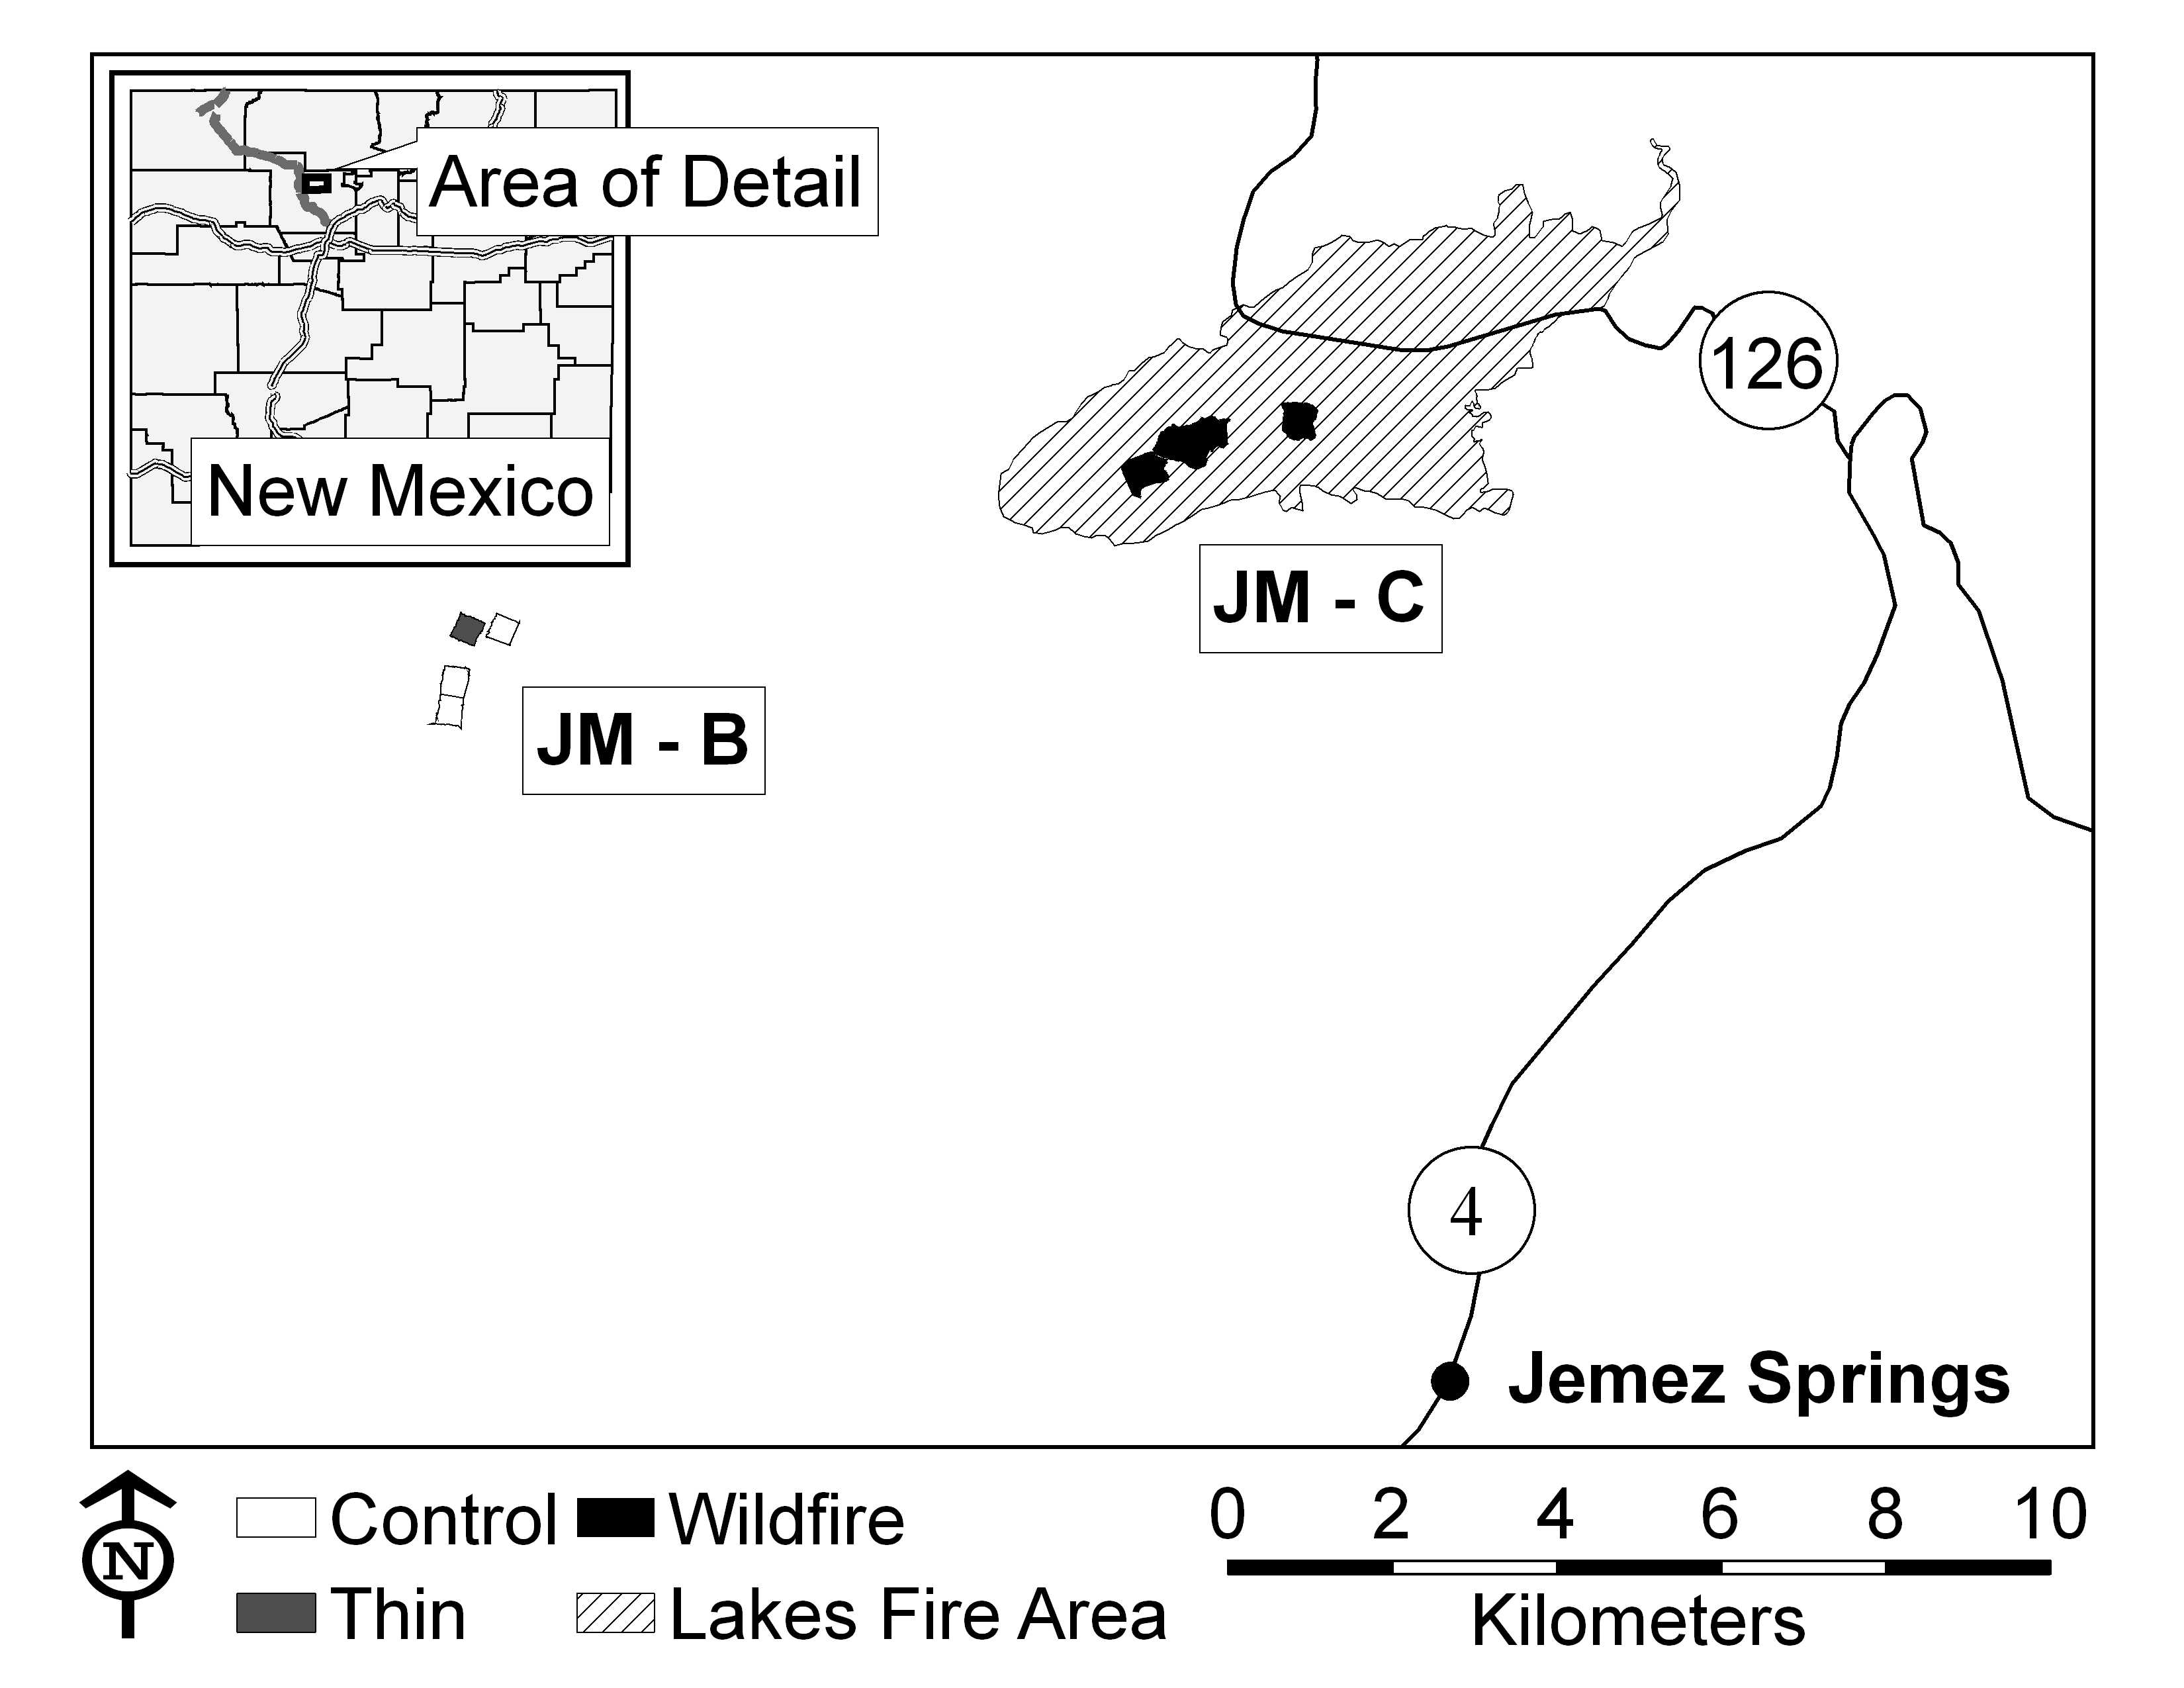
\includegraphics[height=5in,width=6.6in]{Ch13-Multisession/figs/converse_NM_Overview_4.jpg}
\end{center}
\caption{
Central New Mexico Study Area from Converse et al. (2006).
}
\label{fig.studyarea}
\end{figure}


\clearpage





\begin{figure}[htp]
\begin{center}
\includegraphics[height=4.8in,width=6.5in]{Ch13-Multisession/figs/figure_V2.pdf}
\end{center}
\caption{
Abundance estimates for Peromyscus spp. per experimental unit
(with area = 5.0625 ha) for each of 24 groups composed of 8
experimental units in year 1 (groups 1:8), and the same 8
experimental units in year 2 (groups 9:16) and year 3 (groups 17:24)
at the Jemez Mountains Study Area, New Mexico.  Point estimates
(filled circles) are posterior modes, and error bars reflect 95\%
credible intervals. Also shown are the number of individuals
captured per group (open circles).  }
\label{fig.fig1}
\end{figure}


\section{Topics in Multi-Session models}

The thing is this induces a slight bit of {\it dependence} among the
counts but, for even a smallish number of populations , and of
moderate size, the dependence is imperciptable and we think basically
irrelevant from an inference standpoint. 

Over-dispersion. Everyone loves it. Could have normal random effect or
Gamma distribution. 

\subsection{Temporal models }

The case here is we have $g=1,\ldots,G$ samples over time but
individuals are coming and going.
We might capture some individuals over time but we ignore the
individual recaptures across primary periods. (See chapter
\ref{chapt.open}). So instead of modeling the dynamics at the individual
level we just model net change in $N_{g}$.


\subsection{Dependence -- is it a problem?}

{\bf XXX This should probably go in the body of the text or something XXXX}

In time -- ignoring the dependence of $N_{g}$ probably entails a
little {\it loss} of efficiency but should have no effect on anything.
In space, there might be some individuals shared by multiple groups
and we don't think that should cause any bias or anything, even in
statement of uncertainty. So we view these models as pretty generally
useful and relevant.
A few points worht discussing: If you have grids that are in
relatively close proximity you might want to build a model in which
the total state-space is used in the model. i.e., form the union of
the state-spaces and model that. That will be more computationally
tedious but on the other hand it preserves the real landscape and any
interactions that might be affecting grids simultaneously. 


Conceptually we can apply models like this which assume Ng are
independent even if they're not... as long as we dont cear about the
underlying dynamics explictly and also possibly with some loss of
eficiency. 

GROUPS, STRATA, POPULATIONS, ETC...????

\section{Multi-session models in \mbox{\tt secr}  }

We talked about this back in sec. xxx and also in sec. xxxxx....

The {\bf R} package \mbox{\tt secr} (Efford 2011) implements an
estimator for ``multiple sessions'' that could be applied to data from
multiple trap arrays or other meaningfully grouped data.
 The multi-session
model in \mbox{\tt secr} 
arises by an explicit Poisson assumption on $N$, but uses
 a classical likelihood analysis in which the parameters $N_{g}$
are removed from the likelihood by marginalizing the
conditional-on-$N$ likelihood over a Poisson prior.  One advantage of
our Bayesian formulation based on data augmentation which enables
direct implementation in widely available software (WinBUGS, JAGS,
OpenBUGS) is that it is more versatile in terms of the model
specification. For example, here we allowed for multiple
group-specific random effects in the detection model, which is not
accommodated in the \mbox{\tt secr}
package. As another (potential) example, we believe the model could be
extended to open populations (Gardner et al. 2010) without much
difficulty.

\subsection{Ovenbird data in WinBUGS?}

Multi-catch observation model.... it is worth fitting this for sure.

\subsection{Converse data in secr?}

probably leave this out .... too much stuff..... but a simplified
model would run a lot faster in secr I bet.  

\section{Summary and Outlook}


The other context is temporally indexed data -- multi-session or
group-structured models are a simplified type of open model, one
without explicit Markovian dynamics. The models are not incorrect per
se, but just simpler, reduced versions of the more general Markovian
models. We do cover the Markovian models in Chapt. \ref{chapt.open}


SCR data are not
always collected as single isolated studies but, rather, usually a number of
replicate trap arrays are used. Often this is motivated by specific
objectives, e.g., the trap arrays represent experimental replicates,
and oftentimes just to obtain more valid estimates of density by
obtaining a representative sample of space within some region.  Thus
there is a need to combine data from multiple arrays or sites in a
single unified model that accommodates explicit sources of variation
in density among sites.  This is naturally accomplished by developing
an explicit model for variation in $N$, e.g., a Poisson GLM or
similar.

In this paper we extended SCR models to allow for modeling variation
in $N$ with explicit assumptions on $N$. We adopt the data
augmentation strategy from Converse and Royle (2012), and Royle et
al. (2012) and extended this to the spatial capture-recapture
observation model, and applied that model to data from a study of
forest disturbance effects on small mammal populations.  
The framework for combining multiple sites is general and will
work for any kind of SCR observation model.
We demonstrated a multi-catch (ovenbird), single-catch (microtus)
and a bernoulli (simulated data) model.......
Implementation in a Bayesian framework allows for modeling
of individual effects (and hence makes SCR possible) but also
facilitates efficient modeling of nuisance variation via hierarchical
structures (for example, on detection parameters, block effects, or
time effects). However, certain types of models can be fitted in secr
easily, and ...............


Previously people always did ad hoc shit when confronted with
multi-session types of capture-recapture data. They would get Nhats
and do regression on this. For example, 
our small-mammal trapping case study comes from 
Converse et al (2006), who used
a 3 step process to complete the analysis of these data: first a
closed capture-recapture analysis to estimate abundance, second an
analysis of mean maximum distance moved (Wilson and Anderson 1985) to
allow conversion of abundance to density, and third a weighted
regression analysis of the  resulting density estimates. The
weighted analysis was necessary to accomodate the non-zero sampling
covariances resulting from the first 2 steps. The analysis shown
herein is both more streamlined and also integrates the improvements
that spatial capture-recapture methods bring to the estimation of
capture-recapture data. In addition, the Bayesian analysis we present
makes the use of hierarchical structures simple, such as the random effects
for modeling variation in components of detection. Converse
and Royle (2012) showed that the use of random effects for modeling
variation in components of detection provides a good compromise
between model complexity and parsimony, and can result in the lowest root
mean square error in analyses of replicated capture-recapture data.









